\documentclass[11pt]{article}
\usepackage{fullpage}
\usepackage{amsmath}
\usepackage{amssymb}
\usepackage{amsthm}
\usepackage{mathabx}
\usepackage{color}
\usepackage{cancel}
\usepackage{wrapfig}
\usepackage{subcaption}
\usepackage{caption}
\usepackage{xfrac}
\usepackage{algorithm}
\usepackage{algorithmic}
\usepackage{mdframed}
\usepackage{hyperref}
\usepackage{xcolor}
\hypersetup{
  colorlinks,
  linkcolor={red!40!gray},
  citecolor={blue!40!gray},
  urlcolor={blue!70!gray}
}
\usepackage{cleveref}
\def\opt{{\textsc{OPT}_k}}
\def\const{{\mathrm{const}}}
\def\nnz{{\mathrm{nnz}}}
\def\r{\sfrac{\sigma_{\w}^2}{\sigma_{\xib}^2}}
\def\rm{\sfrac{\sigma_{\xib}^2}{\sigma_{\w}^2}}
\def\cmark{\Green{\checkmark}}
\def\xmark{\Red{\large\sffamily x}}
\newcommand{\pdet}{{\mathrm{pdet}}}
\newcommand{\MSPE}[1] {{\mathrm{MSPE}\big[#1\big]}}
\newcommand{\MSE}[1] {{\mathrm{MSE}\big[#1\big]}}
\def\Poisson{{\operatorname{Poisson}}}
\def\PB{{\operatorname{PB}}}
\newcommand{\DP}[1]{\mathcal{DP}^{#1}}
\def\Ic{\mathcal{I}}
\def\Jc{\mathcal{J}}
\def\Mc{\mathcal M}
\def\Ec{\mathcal E}
\def\sr{{\mathrm{sr}}}
\def\ktd{{k^{\underline{d}}}}
\def\Det{{\mathrm{Det}}}
\def\detu{{\widecheck{\mathrm{Det}}_\mu^\gamma}}
\def\deto{{\widehat{\mathrm{Det}}_\mu^\gamma}}
\def\Zu{{\widecheck{Z}_\mu^{\gamma}}}
\def\Zo{{\widehat{Z}_\mu^{\gamma}}}
\def\Zun{{\widecheck{Z}_\mu^{\gamma_n}}}
\def\Zon{{\widehat{Z}_\mu^{\gamma_n}}}
\newcommand{\Er}{\mathrm{Er}}
\newif\ifDRAFT
\DRAFTtrue
\ifDRAFT
\newcommand{\marrow}{\marginpar[\hfill$\longrightarrow$]{$\longleftarrow$}}
\newcommand{\niceremark}[3]
   {\textcolor{red}{\textsc{#1 #2:} \marrow\textsf{#3}}}
\newcommand{\ken}[2][says]{\niceremark{Ken}{#1}{#2}}
\newcommand{\manfred}[2][says]{\niceremark{Manfred}{#1}{#2}}
\newcommand{\michael}[2][says]{\niceremark{Michael}{#1}{#2}}
\newcommand{\michal}[2][says]{\niceremark{Michal}{#1}{#2}}
\newcommand{\feynman}[2][says]{\niceremark{Feynman}{#1}{#2}}
%\usepackage[inline]{showlabels}
\else
\newcommand{\ken}[1]{}
\newcommand{\michael}[1]{}
\newcommand{\michal}[1]{}
\newcommand{\feynman}[1]{}
\fi
\newcommand{\norm}[1]{{\| #1 \|}}

\newcommand{\deff}{d_{\textnormal{eff}}}
\def\ee{\mathrm{e}}
\newcommand\mydots{\makebox[1em][c]{.\hfil.\hfil.}}
\def\Sd{\mathscr{S}_{\!d}}
\newcommand{\dx}{\dxy_{\!\cal X}}
\newcommand{\dxk}{\dxy_{\!\cal X}^k}
\newcommand{\dk}{\dxy^k}
\newcommand{\dxy}{\mathrm{D}}
\def\simiid{\overset{\textnormal{\fontsize{6}{6}\selectfont
i.i.d.}}{\sim}}
%\newcommand{\Dxy}{D_{\!\cal X\!,\cal Y}}
\def\vskx{{\mathrm{VS}_{\!\dx}^k}}
\def\vsk{{\mathrm{VS}_{\!D}^k}}
\def\vskxm{{\mathrm{VS}_{\!\dx}^{k-1}}}
\def\vskm{{\mathrm{VS}_{\!D}^{k-1}}}
\def\vsdx{{\mathrm{VS}_{\!\dx}^d}}
\def\vsd{{\mathrm{VS}_{\!D}^d}}
\newcommand{\vs}[1]{{\mathrm{VS}_{\!D}^{#1}}}
\newcommand{\sigd}{\boldsymbol\Sigma_{\!\dx}}
\def\wols{\w_{\mathrm{LS}}}
\def\wds{\boldsymbol\w_{\!D}^*}
\def\kd{K_{\!\dx}}

\def\poly{{\mathrm{poly}}}
\def\polylog{{\mathrm{polylog}}}
\def\DPP{{\mathrm{DPP}}}
\def\DPPcor{{\DPP_{\!\mathrm{cor}}}}
\def\DPPens{{\DPP_{\!\mathrm{ens}}}}
\newcommand{\DPPreg}[1]{{\DPP_{\!\mathrm{reg}}^{#1}}}
\def\Vol{{\mathrm{VS}}}
\def\Lev{{\mathrm{Lev}}}
\newcommand\todod[1]{\Red{\# DH: #1}}
\newcommand{\explain}[2]{\mathrel{\overset{\makebox[0pt]{\text{\tiny
#1}}}{#2}}}
\def\tot {{\mathrm{tot}}}
\def\checkmark{\tikz\fill[scale=0.4](0,.35) -- (.25,0) --
(1,.7) -- (.25,.15) -- cycle;}
\newcommand{\mnote}[1]{{\bf\large \Magenta{*}}\marginpar{\small \Magenta{#1}}}
\newcommand{\bnote}[1]{{\bf #1}}

\newcommand{\sqrtshort}[1]{{\sqrt{\white{\Big|}\!\!\smash{\text{\fontsize{9}{9}\selectfont$#1$}}}}}
\newenvironment{proofof}[2]{\par\vspace{2mm}\noindent\textbf{Proof of {#1} {#2}}\ }{\hfill\BlackBox}
\newcommand{\sets}[2]
{{\hspace{-0.3mm}[\hspace{-0.3mm}#1\hspace{-0.3mm}]\hspace{-0.3mm}\choose
\hspace{-0.3mm}#2\hspace{-0.3mm}}}
\DeclareMathOperator{\sgn}{\textnormal{sgn}}
\DeclareMathOperator{\adj}{\textnormal{adj}}
\def\Rb{{\mathbf{R}}}
\DeclareMathOperator{\ws}{\widetilde{\w}}
\newcommand{\inote}[1]{{\bf {#1}}}
\def\xib{\boldsymbol\xi}
\def\Sigmab{\mathbf{\Sigma}}
\def\Sigmabh{\widehat{\Sigmab}}
\def\Sigmabt{\widetilde{\Sigmab}}
\def\S{\mathbf{S}}
\def\T{\mathbf{T}}
\def\xt{\tilde{x}}
\def\xbt{\widetilde{\x}}
\def\xbh{\widehat{\x}}
\def\ubh{\widehat{\u}}
\def\dom {{\mathrm{dom}}}
\def\val {{\mathrm{val}}}
\def\out {{\mathrm{out}}}
\def\iin  {{\mathrm{iin}}}
\def\s {\mathbf{s}}
\def\q {\mathbf{q}}
\def\qt{\tilde{q}}
\def\itld {j}
\def\ubt {\tilde{\u}}
\def\n{\{1..n\}}
\def\cb {\mathbf{c}}
\def\cW{\mathcal W}
\def\Xt{\widetilde{X}}
\def\Dbt{\widetilde{\D}}
\def\xtb{\tilde{\mathbf{x}}}
\def\ytb{\tilde{\mathbf{y}}}
\def\Xtb{\widetilde{\mathbf{X}}}
\def\Xbb{\overline{\X}}
\def\Xb{{\bar{\X}}}
\def\ybb{\overline{\y}}
\def\f{{\mathbf{f}}}
\def\g{{\mathbf{g}}}
\def\fbb{{\overline{\f}}}
\def\fb{{\overline{f}}}
\def\Xc{\mathcal{X}}
\def\W{\mathbf W}
\def\L{\mathbf{L}}
\def\Rb{\mathbf R}
\def\Pc{\mathcal{P}}
\def\Nc{\mathcal{N}}
\def\Pt{\widetilde{P}}
\def\Hc{\mathcal{H}}
\def\Wc{\mathcal{W}}
\def\Cc{\mathcal{C}}
\def\p{\mathbf p}
%\def\r{\mathbf r}
\def\Y{\mathbf Y}
\def\H{\mathbf H}
\def\K{\mathbf K}
\def\Kh{\widehat{K}}
\def\Kbh{{\widehat{\K}}}
\def\Q{\mathbf Q}
\def\Qbar{{\bar{\mathbf Q}}}
\def\Ytb{\widetilde{\mathbf{Y}}}
\def\c{{n-d\choose s-d}}
\DeclareMathOperator{\Proj}{Proj}
\newcommand{\Span}{\mathrm{span}}
\newcommand{\ofsubt}[1]{\mbox{\scriptsize \raisebox{0.25pt}{$(#1)$}}}
%\raisebox{0.5pt}{$($}}#1\mbox{\tiny \raisebox{0.5pt}{$)$}}}
\newcommand{\ofsub}[1]{\mbox{\small \raisebox{0.0pt}{$(#1)$}}}
%\newcommand{\ofsubb}[1]{\mbox{\footnotesize \raisebox{0.5pt}{$(#1)$}}}
%\newcommand{\ofsub}[1]{(#1)}
%\newcommand{\ofsub}[1]{\mbox{\tiny$|$\hspace{-0.5pt}\raisebox{-0.5pt}{$#1$}}}
\newcommand{\of}[2]{{#1{\!\ofsub{#2}}}}
\newcommand{\oft}[2]{{#1{\!\ofsubt{#2}}}}
\newcommand{\fof}[2]{{#1({#2})}}
\newcommand{\yof}[2]{{#1{\ofsub{#2}}}}
%\newcommand{\yofb}[2]{{#1{\ofsubb{#2}}}}
\newcommand{\lazy}{FastRegVol}
\newcommand{\volsamp}{RegVol}

\newcommand{\Sm}{{S_{-i}}}
\newcommand{\Sp}{{S_{+i}}}
\ifx\BlackBox\undefined
\newcommand{\BlackBox}{\rule{1.5ex}{1.5ex}}  % end of proof
\fi
%\renewcommand{\dagger}{+}
\DeclareMathOperator*{\argmin}{\mathop{\mathrm{argmin}}}
\DeclareMathOperator*{\argmax}{\mathop{\mathrm{argmax}}}
\DeclareMathOperator*{\diag}{\mathop{\mathrm{diag}}}
\def\x{\mathbf x}
\def\y{\mathbf y}
\def\ybh{\widehat{\mathbf y}}
\def\ybb{\bar{\mathbf y}}
\def\xbb{\bar{\mathbf x}}
\def\yb{{\bar y}}
\def\ybt{\widetilde{\mathbf y}}
\def\yh{\widehat{y}}
\def\yhb{\widehat{\y}}
\def\yt{\widetilde{y}}
\def\z{\mathbf z}
\def\a{\mathbf a}
\def\b{\mathbf b}
\def\w{\mathbf w}
\def\v{\mathbf v}
\def\m{\mathbf m}
\def\wbh{\widehat{\mathbf w}}
\def\wh{\widehat{\mathbf w}}
\def\vbh{\widehat{\mathbf v}}
\def\wbt{\widetilde{\mathbf w}}
\def\e{\mathbf e}
\def\zero{\mathbf 0}
\def\one{\mathbf 1}
\def\u{\mathbf u}
\def\ubbar{\bar{\mathbf u}}
\def\f{\mathbf f}
\def\ellb{\boldsymbol\ell}

\def\X{\mathbf X}
\def\Xs{\widetilde{\X}}
\def\B{\mathbf B}
\def\A{\mathbf A}
\def\C{\mathbf C}
\def\U{\mathbf U}
\def\Ubt{\widetilde{\mathbf U}}
\def\Ubh{\widehat{\mathbf U}}
\def\Ubbar{\bar{\mathbf U}}
\def\F{\mathbf F}
\def\D{\mathbf D}
\def\V{\mathbf V}
\def\M{\mathbf M}
\def\Mh{\widehat{\mathbf M}}
%\def\S{\mathbf S}
\def\Stb{\widetilde{\mathbf{S}}}
\def\Sbh{\widehat{\mathbf{S}}}
\def\St{\widetilde{\S}}
\def\Sh{\widehat{S}}
\def\Sc{\mathcal{S}}
\def\Fc{\mathcal{F}}
\def\Vc{\mathcal{V}}
\def\Bc{\mathcal{B}}
\def\Dc{\mathcal{D}}
\def\Z{\mathbf Z}
\def\Zbh{\widehat{\mathbf Z}}
\def\Zbt{\widetilde{\mathbf Z}}
\def\Abh{\widehat{\mathbf A}}
\def\I{\mathbf I}
\def\Ic{\mathcal I}
\def\II{\mathbf {I \!\,I}}
%\def\II{\boldsymbol {\mathbb I}}
\def\A{\mathbf A}
\def\P{\mathbf P}
\def\Ph{\widehat{\mathbf P}}
\def\cP{\mathcal P}
\def\cR{\mathcal R}
\def\Xt{\widetilde{\mathbf{X}}}
\def\Xh{\widehat{\mathbf{X}}}
\def\Rh{\widehat{R}}
\def\Ot{\widetilde{O}}
\def\At{\widetilde{\A}}


\def\E{\mathbb E}
\def\R{\mathbb R}
\def\N{\mathbb N}
\def\Pr{\mathrm{Pr}}
%\def\C{\mathbb C}
\def\tr{\mathrm{tr}}
\def\Sbar{{\bar{S}}}
\def\cS{{\mathcal{S}}}
\def\Tbar{{\bar{T}}}
\def\Tt{{\widetilde{T}}}
\def\rank{\mathrm{rank}}
\def\Prob{\mathrm{Prob}}
\def\Var{\mathrm{Var}}
\def\Xinv{(\X^\top\X)^{-1}}
\def\XinvS{(\X_S\X_S^\top)^{-1}}
\def\ABinvS{(\A_S\B_S^\top)^{-1}}
\def\ABinv{(\A\B^\top)^{-1}}
\def\xinv{\x_i^\top\Xinv\x_i}
\def\Xinvr{(\lambda\I+\X_{-1}^\top\X_{-1})^{-1}}
\def\pdet{\mathrm{pdet}}
\newcommand{\vol}{\mathrm{vol}}
%\newcommand{\defeq}{:=}
\newcommand{\defeq}{\stackrel{\textit{\tiny{def}}}{=}}
\newcommand{\di}{{[d+1]_{-i}}}
\newcommand{\cov}{\mathrm{cov}}
\let\origtop\top
\renewcommand\top{{\scriptscriptstyle{\origtop}}} % this makes transpose not so big

\definecolor{silver}{cmyk}{0,0,0,0.3}
\definecolor{yellow}{cmyk}{0,0,0.9,0.0}
\definecolor{reddishyellow}{cmyk}{0,0.22,1.0,0.0}
\definecolor{black}{cmyk}{0,0,0.0,1.0}
\definecolor{darkYellow}{cmyk}{0.2,0.4,1.0,0}
\definecolor{orange}{cmyk}{0.0,0.7,0.9,0}
\definecolor{darkSilver}{cmyk}{0,0,0,0.1}
\definecolor{grey}{cmyk}{0,0,0,0.5}
\definecolor{darkgreen}{cmyk}{0.6,0,0.8,0}
\newcommand{\Red}[1]{{\color{red}  {#1}}}
\newcommand{\Purple}[1]{{\color{purple}  {#1}}}
\newcommand{\Magenta}[1]{{\color{magenta}{#1}}}
\newcommand{\Green}[1]{{\color{darkgreen}  {#1}}}
\newcommand{\Blue}[1]{\color{blue}{#1}\color{black}}
\newcommand{\Orange}[1]{\textcolor{orange}{#1}\color{black}}
\newcommand{\Brown}[1]{{\color{brown}{#1}\color{black}}}
\newcommand{\Grey}[1]{{\color{grey}{#1}\color{black}}}
\newcommand{\white}[1]{{\textcolor{white}{#1}}}
\newcommand{\yellow}[1]{{\textcolor{reddishyellow}{#1}}}
\newcommand{\darkYellow}[1]{{\textcolor{darkYellow}{#1}}}
\newcommand{\grey}[1]{{\textcolor{grey}{#1}}}

\DeclareMathOperator{\half}{\frac{1}{2}}

\ifx\proof\undefined
\newenvironment{proof}{\par\noindent{\bf Proof\ }}{\hfill\BlackBox\\[2mm]}
\fi

\ifx\theorem\undefined
\newtheorem{theorem}{Theorem}
\fi

\ifx\example\undefined
\newtheorem{example}{Example}
\fi

\ifx\condition\undefined
\newtheorem{condition}{Condition}
\fi
\ifx\property\undefined
\newtheorem{property}{Property}
\fi

\ifx\lemma\undefined
\newtheorem{lemma}{Lemma}
\fi

\ifx\proposition\undefined
\newtheorem{proposition}{Proposition}
\fi

\ifx\remark\undefined
\newtheorem{remark}{Remark}
\fi

\ifx\corollary\undefined
\newtheorem{corollary}{Corollary}
\fi

\ifx\definition\undefined
\newtheorem{definition}{Definition}
\fi

\ifx\conjecture\undefined
\newtheorem{conjecture}{Conjecture}
\fi

\ifx\axiom\undefined
\newtheorem{axiom}{Axiom}
\fi

\ifx\claim\undefined
\newtheorem{claim}{Claim}
\fi

\ifx\assumption\undefined
\newtheorem{assumption}{Assumption}
\fi

\ifx\condition\undefined
\newtheorem{condition}{Condition}
\fi



\title{Exact expressions for random projections: Open problems}
\author{Micha{\l} Derezi\'nski, UC Bekeley}
% \setlength{\parindent}{0cm}
% \setlength{\parskip}{0mm}

\begin{document}
\maketitle

\section{Main results}
Consider a large $m\times n$
matrix $\A$. A data-oblivious sketch of size $k$ is the matrix $\S\A$,
where $\S$ is a $k\times m$ random matrix such that
$\E[\frac1k\S^\top\S]=\I$, and whose distribution does not
depend on $\A$.
\begin{theorem}\label{t:main}
Let $\S$ be a sketch of size $k$ with i.i.d.~mean-zero sub-Gaussian entries and let
  $r=\|\A\|_F^2/\|\A\|^2$ be the stable rank of $\A$.  If
  we let $\rho = r/k$ be a fixed constant larger than $1$, then
  \begin{align*}
    (1-\epsilon)\,\bar\P_{\!\perp}\preceq\E[\P_{\!\perp}]\preceq
    (1+\epsilon)\,\bar\P_{\!\perp}\quad\text{for}\quad \epsilon =
    O(\tfrac1{\sqrt r}),
  \end{align*}
  where $\P_{\!\perp} :=\I - (\S\A)^\dagger\S\A,$ and $\bar\P_{\!\perp}:=(\gamma\A^\top\A +
  \I)^{-1}$, for $\gamma>0$  s.t. $\tr\,\bar\P_{\!\perp} = n-k$.
\end{theorem}
% \begin{theorem}\label{t:main-tech}
% Let $\P_\perp = \I - \X^\dagger \X$ for $\X = \Z\Sigmab^{\frac12}$,
% where $\Z \in \mathbb R^{k\times n}$ has i.i.d.~$K$-sub-Gaussian rows with zero mean and identity covariance, and
% $\Sigmab$ is an $n\times n$ positive semi-definite matrix. Define: 
% \begin{align*}
% \bar\P_\perp= (\gamma\Sigmab + \I)^{-1},\quad\text{such that}\quad\tr\,\bar\P_\perp=n-k.
% \end{align*}
% Let $r =\tr(\Sigmab)/\|\Sigmab\|$
% be the stable rank of
% $\Sigmab^{\frac12}$ and fix $\rho=r/k > 1$. There exists a constant
% $C_{\rho}>0$, depending only on $\rho$ and $K$, such that if $r\geq
% C_\rho$, then
% \begin{align}
% \Big(1-\frac {C_\rho}{\sqrt
%   r}\Big)\cdot\bar\P_\perp\preceq\E[\P_\perp]\preceq
%   \Big(1+\frac {C_\rho}{\sqrt r}\Big)\cdot\bar\P_\perp.
% \end{align}
% \end{theorem}
\begin{corollary} %[low-rank approximation]
  \label{c:low-rank}
Let $\sigma_i$ be the singular values of $\A$. Under the assumptions of Theorem \ref{t:main}, we have:\vspace{-1mm}
  \begin{align*}
    \E\big[\|\A-\A\P\|_F^2\big] \ \overset\epsilon\simeq\ 
    k/\gamma
\quad \text{for \ $\gamma>0$ \ s.t. \ } \sum_{i}\frac{\gamma\sigma_i^2}{\gamma\sigma_i^2+1} = k.
  \end{align*}
\end{corollary}
\begin{corollary}\label{c:kaczmarz}
Let $\x^*$ be the unique solution of $\A\x^*=\b$ and consider
  the iterative algorithm:
  \begin{align*}
    \x^{t+1} = \argmin_\x\|\x-\x^t\|^2\quad\textnormal{subject to}\quad\S_t\A\x=\S_t\b.
  \end{align*}
Under the assumptions of Theorem \ref{t:main}, with $r=\|\A\|_F^2/\|\A||^2$, we have:
  \begin{align*}
    \E\big[\x^{t+1}-\x^*\big] \overset\epsilon\simeq 
    (\gamma\A^\top\A+\I)^{-1}\,\E\big[\x^t-\x^*\big]
    \quad\text{for}\quad\epsilon=O(\tfrac1{\sqrt r}). 
  \end{align*}
Moreover, we obtain the following worst-case convergence guarantee:
\begin{align}
  \E\big[\|\x^{t+1}-\x^*\|^2\big]
  \leq \big(1-
  (\bar\kappa-\epsilon)\big)\,\E\big[\|\x^{t}-\x^*\|^2\big],
  \quad\text{where}\quad
  \bar\kappa = \frac{\sigma_{\min}^2(\A)}{\sigma_{\min}^2(\A)+1/\gamma}.\label{eq:worst-case}
\end{align}
\end{corollary}


\section{Open questions}
\subsection{Extend the result beyond the stable rank}
\begin{figure}[h]
  \centering
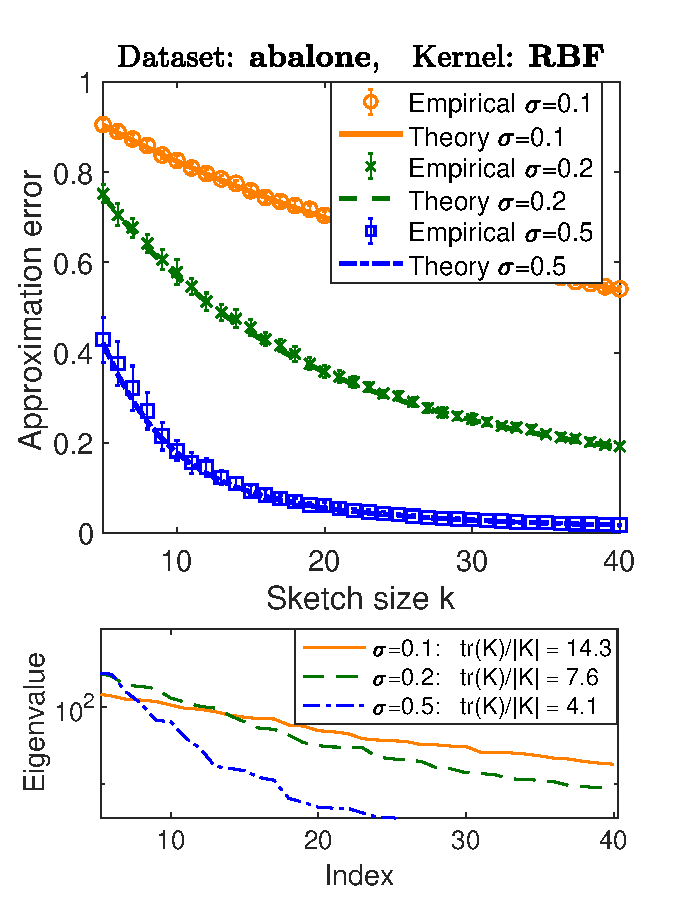
\includegraphics[width=.4\textwidth]{../equivalents_nips/abalone-nystrom}\nobreak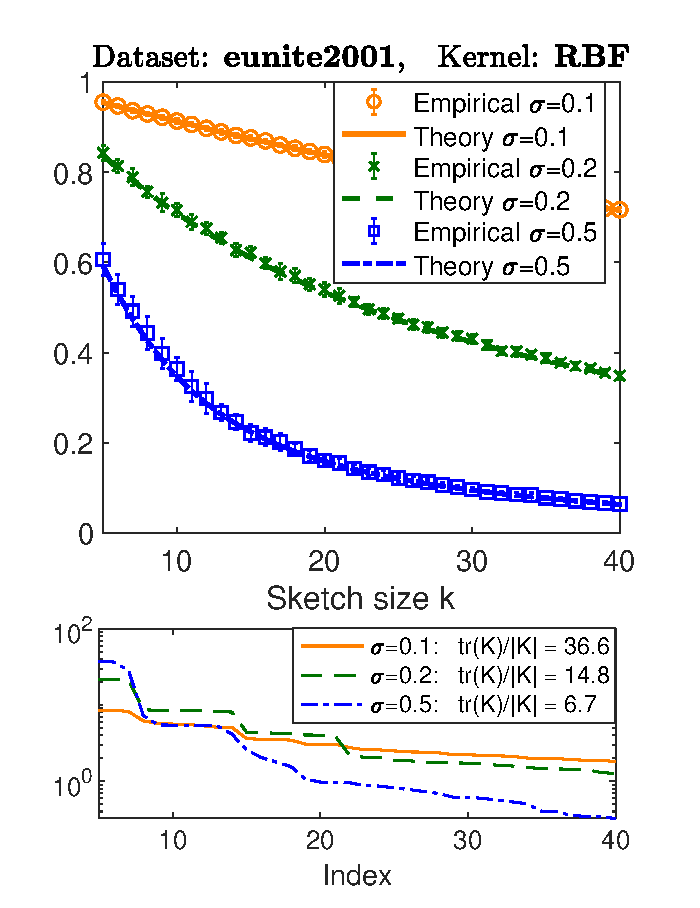
\includegraphics[width=.4\textwidth]{../equivalents_nips/eunite-nystrom}
\caption{
Theoretical predictions of low-rank approximation error of a Gaussian
sketch along with spectral decay profiles and stable rank of the
matrices. Note that we use a kernel matrix notation $\K$, which can be
converted to the data matrix $\A=\K^{\frac12}$. 
}
%\vspace{-5mm}
\label{f:explicit}
\end{figure}

In Figure \ref{f:explicit}, we observe that, for standard spectral
decay profiles, the surrogate expression
of low-rank approximation error (see Corollary \ref{c:low-rank}) is
accurate even when $k$ is larger than the stable rank of the data
matrix. In particular, it seems that as long as the spectral decay
does not have a sudden drastic drop around $k$, the surrogate
expressions are accurate. This, to a certain degree, can also be
observed for the expected residual projection, i.e. $\E[\P_{\perp}]$.
Thus, we raise a number of questions:
\begin{enumerate}
  \item Under what conditions on the spectral decay can we let $k>r$
    and still have the surrogate expressions be asymptotically
    consistent (i.e., error decays to zero)?
  \item Under what conditions on the spectral decay can we ensure a
    $\frac12$-approximation for surrogate expressions, i.e., that
    $\frac12\bar\P_{\perp}\preceq\E[\P_{\perp}]\preceq\frac32\bar\P_{\perp}$?
  \item Under what conditions on the spectral decay can we ensure a
    $\frac12$-approximation for the low-rank approximation error,
    i.e., as in Corollary \ref{c:low-rank}, with $\epsilon=\frac12$ (a
    strictly weaker guarantee)?
\end{enumerate}
%\subsection{Extend the result to other sketches, e.g., SRHT}

\subsection{Expectation of non-residual projection, $\E[\P]$, where
  $\P=(\S\A)^\dagger\S\A$}\label{s:non-residual}
Our surrogate expression for $\E[\P]$ has the form
$\bar\P:=\gamma\Sigmab(\gamma\Sigmab+\I)^{-1}$. Using the guarantees
for the residual projection, we can immediately obtain the following:
\begin{align*}
(1-\epsilon)\bar\P - \epsilon \I\preceq \E[\P]\preceq (1+\epsilon)\bar\P + \epsilon\I.
\end{align*}
This is an additive approximation gurantee, which is very
weak for small eigenvalues of $\E[\P]$. Note that unlike the surrogate
expression for the \emph{residual} projection, $\bar\P$ can have very small
eigenvalues, which presents additional challenges in the
analysis. Because of this, we expect some dependence of the guarantees
on the ambient dimension $n$, and possibly on the condition number.

\begin{conjecture}\label{h:non-residual}
Let $\A$ be an $m\times n$ matrix with stable rank
  $r=\|\A\|_F^2/\|\A\|^2$, such that $n/r\leq\tau$ and $r/k\geq\rho$ for
 fixed constants  $\tau,\rho>1$. Given any sketch $\S$ of size $k$ with
  i.i.d.~mean-zero sub-Gaussian entries, there is an event $E$ such
  that:
\begin{align*}
  \Pr(E)\geq 1-\ee^{-\Theta(r)}\quad\text{and}\quad
  (1-\epsilon)\,\bar\P\preceq\E[\,\P\mid E\,]
  \preceq(1+\epsilon)\,\bar\P\quad\text{for}\quad
  \epsilon=O(\tfrac1{\sqrt r}),
\end{align*}
where $\P:= (\S\A)^\dagger\S\A,$ and
$\bar\P:=\gamma\A^\top\A(\gamma\A^\top\A + \I)^{-1}$,
for $\gamma>0$  such that $\tr\,\bar\P= k$.
\end{conjecture}

\noindent
The event $E$ is used to avoid dependence on the
condition number of $\A$. This seems to be necessary for
discrete-valued sketches (e.g., Rademacher), but it is likely avoidable for the Gaussian sketch.

\subsection{Expectation of incomplete projection,
  $\E[\H]$, where $\H=\S^\top(\S\A\A^\top\S^\top)^\dagger\S$} 
Note that the incomplete projection is related to the projection
matrix as follows:
\begin{align*}
  \P = (\S\A)^\dagger\S\A =
  \A^\top\S^\top(\S\A\A^\top\S^\top)^\dagger\S\A = \A^\top\H\A.
\end{align*}
This quantity appears in certain optimization methods such as Sketched
Newton-Raphson \cite{sketched-newton-raphson}.
Our surrogate expression for $\E[\H]$ should have the form
\begin{align*}
  \E[\H]\ \simeq\ \bar\H:=(\A\A^\top+\tfrac1\gamma\I)^{-1}.
\end{align*}

\begin{conjecture}
  Let $\S$ be a sketch of size $k$ with i.i.d.~mean-zero sub-Gaussian entries and let
  $r=\|\A\|_F^2/\|\A\|^2$ be the stable rank of $\A$.  If
$\rho = r/k>1$ is a constant, then for
  any $z\neq 0$
  \begin{align*}
    (1-\epsilon)\,\bar\H\preceq\E[\H]\preceq
    (1+\epsilon)\,\bar\H\quad\text{with}\quad \epsilon =
    O(\tfrac1{\sqrt r}),
  \end{align*}
  where $\H := \S^\top(\S\A\A^\top\S^\top)^\dagger\S$
  and $\bar\H:=(\A\A^\top+\frac1\gamma\I)^{-1}$, for $\gamma>0$ such
  that $\tr\,\A^\top\bar\H\A = k$.
\end{conjecture}


\subsection{Higher-order corrections for ill-conditioned matrices}

\begin{figure}[h]
  \centering
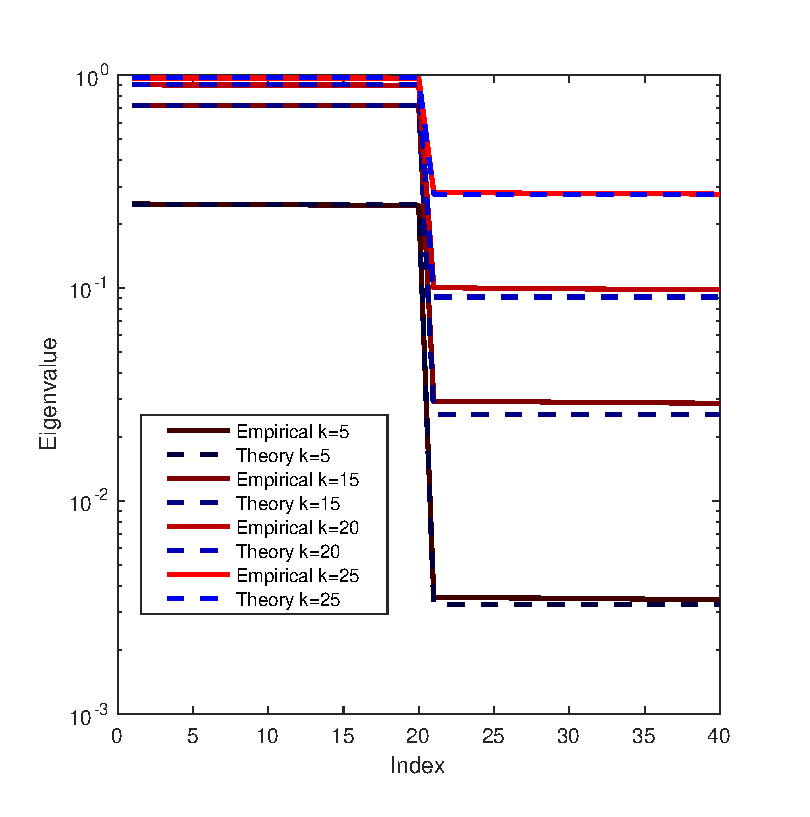
\includegraphics[width=.4\textwidth]{higher}\nobreak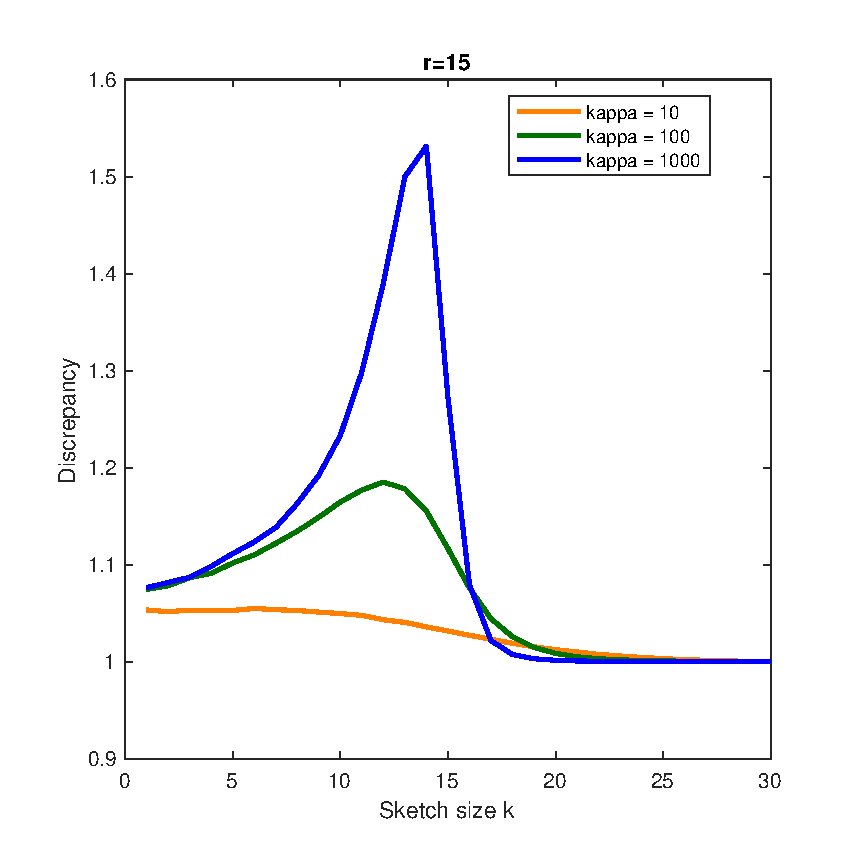
\includegraphics[width=.4\textwidth]{discrepancy}
\caption{}
%\vspace{-5mm}
\label{f:higher-svd}
\end{figure}


The surrogate expression proposed in Theorem \ref{t:main} does not appear
to be correct when the spectrum of $\A$ contains a sharp drop. To
analyze this, consider the following simple example, where $\A^\top\A
= \diag(1,...,1,\kappa^{-1},...,\kappa^{-1})$ for some $\kappa\gg
1$. We can compare the surrogate expression $\bar\P$ with the expected
projection $\E[\P]$ for $\P=(\S\A)^\dagger\S\A$ (similar
observations follow for $\P_{\perp}$), when using a Gaussian
sketch. Note that for the Gaussian sketch, if $\A^\top\A$ is diagonal,
then so are $\E[\P]$ and $\bar\P$, so we can focus on comparing just the
spectrum of both matrices. This is shown in Figure~\ref{f:higher-svd}
(left), where we let $n=40$ and $r\approx 20$, with $\kappa=100$. We
observe that when $k\approx r$, then there is a discrepancy between
the surrogate and the expectation, particularly noticable for the
small eigenvalues. The relative error of the surrogate estimate for
the small eigenvalues as a function of $k$ is shown in Figure
\ref{f:higher-svd} (right), showing that the peak of the error occurs
as $k$ gets close to $r$ (the location of the peak is less than $r$,
but it approaches $r$ as $\kappa$ grows).

Note that this phenomenon presents itself already in the simple case
where $k=1$ and we let
$\A^\top\A=\diag(1,\kappa^{-1},...,\kappa^{-1})$. In this case, our
goal is to find a surrogate expression for a rank-one projection, so
we can formulate the following basic open problem:

\paragraph{Open problem:} Let
$\A=\diag(1,\kappa^{-\frac12},...,\kappa^{-\frac12})$ be an $n\times
n$ matrix, and define $\z\sim\Nc(\zero,\I)$. Find a surrogate
expression $\bar\P_{\kappa,n}$ such that:
\begin{align*}
  \lambda_i\Bigg(\E\bigg[\frac{\A^\top\z\z^\top\A}{\z^\top\A^\top\A\z}\bigg]\Bigg)
  \simeq \lambda_i\big(\bar\P_{\kappa,n}\big)\quad\text{for all $i$}\quad\text{as}\quad \kappa,n\rightarrow\infty.
\end{align*}

\subsection{Upper/lower bounds for the extreme eigenvalues}
\begin{figure}[h]
  \centering
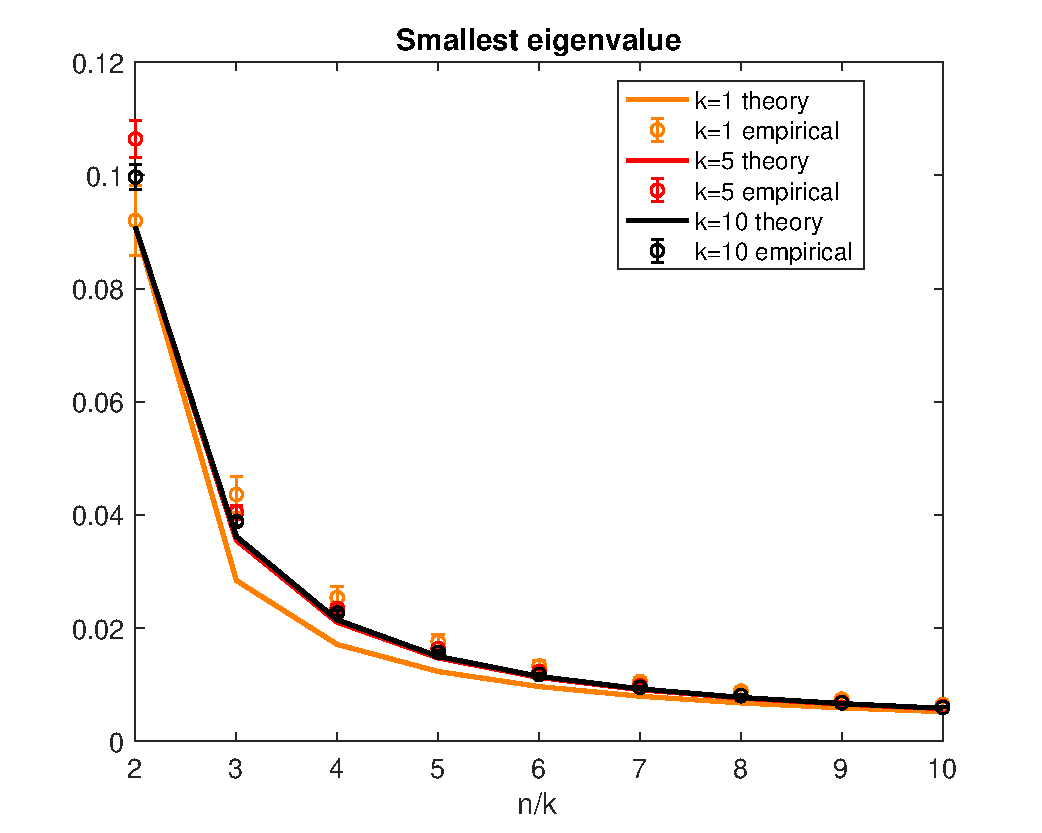
\includegraphics[width=.4\textwidth]{lambda_min}\nobreak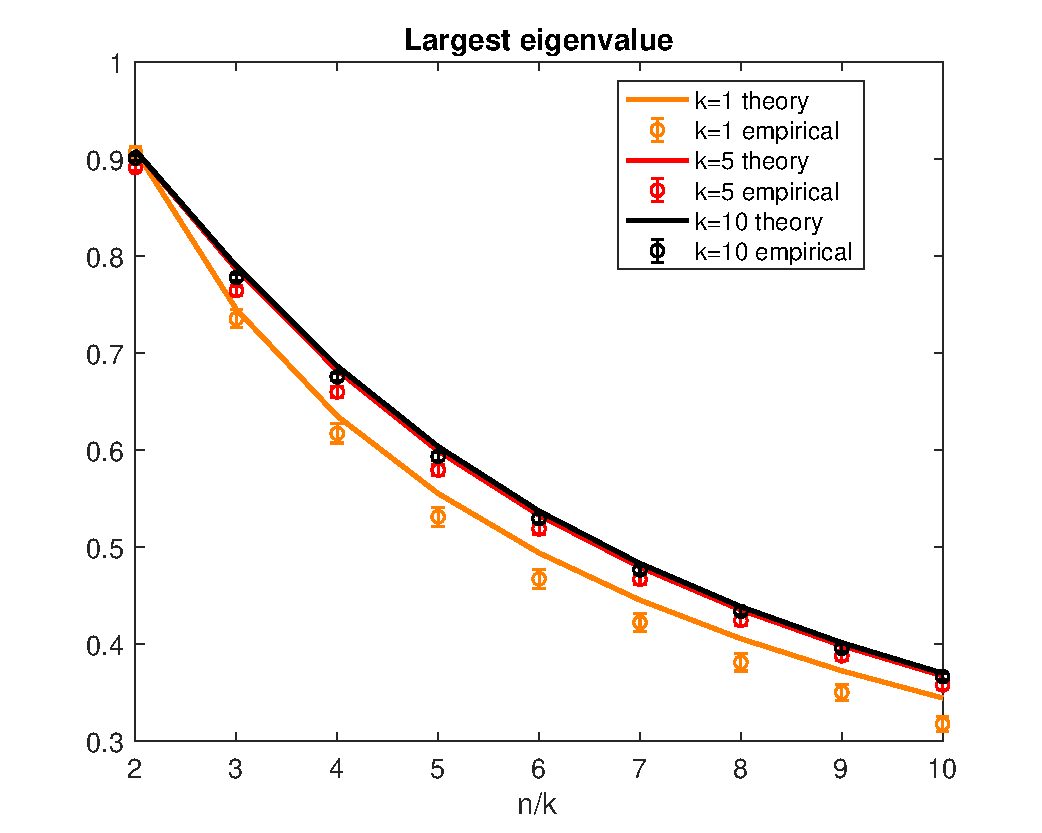
\includegraphics[width=.4\textwidth]{lambda_max}
\caption{}
%\vspace{-5mm}
\label{f:extreme}
\end{figure}


As observed in Figure \ref{f:higher-svd}, even when there is a
significant discrepancy between the eigenvalues of $\E[\P]$ and the
corresponding surrogate expressions, the extreme eigenvalues of
$\bar\P$ provide upper/lower bounds for the extreme eigenvalues of
$\E[\P]$. This has been consistently observed empirically for the Gaussian sketch
regardless of the spectral decay (see Figure \ref{f:extreme}).

\begin{conjecture}\label{h:extreme}
Let $\A$ be an $m\times n$ matrix. For a sketch $\S$ of any size $k$ with
  i.i.d.~standard normal entries we have:
\begin{align*}
  \lambda_{\min}(\bar\P)\leq \lambda_{\min}(\E[\P])\leq
  \lambda_{\max}(\E[\P])\leq \lambda_{\max}(\bar\P),
\end{align*}
where $\P= (\S\A)^\dagger\S\A,$ and
$\bar\P=\gamma\A^\top\A(\gamma\A^\top\A + \I)^{-1}$,
for $\gamma>0$  such that $\tr\,\bar\P= k$.
\end{conjecture}

\noindent
Note that the conjecture is very broad in that it does not require any
assumptions on $\A$ or on the sketch size $k$, because no
example has been found where the statement would be violated. It may
be worthwhile to look for such counter-example.
Further, it is possible that the conjecture also extends to other
sub-Gaussian sketches, or even beyond, although this has not been
verified empirically.

\subsection{Further convergence analysis of Gaussian Kaczmarz method}

The convergence guarantee given in Corollary \ref{c:kaczmarz} invites
the following directions for future work:
\begin{enumerate}
\item  The worst-case convergence rate depends on the smallest
  eigenvalue of $\E[\P]$ so we only have a weak additive
  approximation, which is vacuous when that eigenvalue is small
  enough.
  Can we avoid replace the additive approximation with multiplicative
  one, or eliminate it altogether?
\item The expected trajectory depends on the expected direction of
  $\E[\x^t-\x^*]$. A priori, this direction could match the smallest
  eigenvalue of $\E[\P]$. Is there a way to precondition the
  problem in such a way as to avoid this?
\end{enumerate}
Improving the worst-case convergence  is closely related to proving
Conjectures \ref{h:non-residual} and \ref{h:extreme}. In particular, if Conjecture \ref{h:extreme} is
true, then this eliminates \emph{any} dependence on the approximation
accuracy of the surrogate expressions and leads to a clean statement.
\begin{conjecture}[Corollary of Conjecture \ref{h:extreme}]
Let $\x^*$ be the unique solution of $\A\x^*=\b$ and consider
  the iterative algorithm:
  \begin{align*}
    \x^{t+1} = \argmin_\x\|\x-\x^t\|^2\quad\textnormal{subject to}\quad\S_t\A\x=\S_t\b.
  \end{align*}
Then, the following convergence guarantee holds:
\begin{align}
  \E\big[\|\x^{t+1}-\x^*\|^2\big]
  \leq (1-\bar\kappa)\,\E\big[\|\x^{t}-\x^*\|^2\big],
  \quad\text{where}\quad
  \bar\kappa = \frac{\sigma_{\min}^2(\A)}{\sigma_{\min}^2(\A)+1/\gamma}.
\end{align}
\end{conjecture}
Similar but weaker guarantee can be obtained as a corollary of
Conjecture \ref{h:non-residual}. There, we still suffer from the
approximation parameter $\epsilon$, but the dependence is now
multiplicative instead of additive, which means that the result is non-vacuous
even when the smallest eigenvalue is very small.



\subsection{High-probability guarantees and the spectral norm
error} 

In addition to analyzing the low-rank approximation error using the
Frobenius norm, a large body of literature has also considered other
norms, and particularly the spectral norm \cite{tropp2011structure}:
\begin{align*}
  \text{(spectral norm error)}\quad \|\A-\A\P\| = \|\A\P_{\perp}\|.
\end{align*}
In addition to analysis of the low-rank approximation error, the above
quantity also appears in the analysis of certain randomized iterative
algorithms, such as the one proposed by \cite{lacotte2019high}.

Note that while the Frobenius norm error depends linearly on the residual projection,
i.e., $\|\A\-\A\P\|_F^2 = \tr(\A^\top\A\P_{\perp})$, the spectral norm
depends on it in a non-linear fashion. As a result, the analysis of
expected residual projection does not 
apply directly. Instead, one could hope to obtain high-probability
guarantees on the residual projection, which can then be used to
estimate the spectral norm error.

\paragraph{Open problem.} Let $r$ be the stable rank of $\A$. Show
that for any fixed vector $\x\in\R^n$, we have:
\begin{align*}
  \x^\top\P_{\!\perp}\x\ \overset\epsilon\simeq\ \x^\top(\gamma\Sigmab+\I)^{-1}\x\quad\text{with probability $1-\ee^{-cr}$}.
  \end{align*}

\subsection{Deterministic equivalents for matrix resolvents via 
  stable rank conditions}
Standard random matrix theory analysis focuses on constructing
deterministic equivalents for the resolvent matrix, defined as
follows:
\begin{align*}
  \Q(z) = (\A^\top\S^\top\S\A + z\I)^{-1}\quad\text{for}\quad z\in\mathbb{C}.
\end{align*}
The residual projection matrix which we analyze can be obtained via
the following limit:
\begin{align*}
  \P_{\!\perp}= \I - (\S\A)^\dagger\S\A =  \lim_{z\rightarrow 0}\ z\,\Q(z).
\end{align*}
Many of our results and conjectures can be naturally extended so that
they are also formulated for the resolvent matrices. The obtained
statements should be of independent interest in this context, because
of our use of stable rank to control the spectral properties of the
matrix $\A$ (as opposed to using the condition number, or bounding $z$
away from zero). For example, the following conjecture should follow
similarly as our main result.
\begin{conjecture}
  Let $\S$ be a sketch of size $k$ with i.i.d.~mean-zero sub-Gaussian entries and let
  $r=\|\A\|_F^2/\|\A\|^2$ be the stable rank of $\A$.  If
$\rho = r/k>1$ is a constant, then for
  any $z\neq 0$
  \begin{align*}
    (1-\epsilon)\,\bar\Q(z)\preceq\E[\Q(z)]\preceq
    (1+\epsilon)\,\bar\Q(z)\quad\text{with}\quad \epsilon =
    O(\tfrac1{\sqrt r}),
  \end{align*}
  where $\Q(z) := (\A^\top\S^\top\S\A + z\I)^{-1}$ and $\bar\Q(z):=(\gamma\A^\top\A +
  z\I)^{-1}$.
\end{conjecture}

\noindent
This prompts the question whether or not the conjecture leads to
a novel variant of asymptotic spectral analysis for random matrices, for example, one where we do
not require the limiting spectral distribution to be bounded away from
zero. Also, similarly as in the case of residual projection, we can
ask whether or not the results can be extended beyond the stable rank.

Another motivation for analyzing resolvents is that they naturally
arise when analyzing the bias of sketching for $l_2$-regularized
second-order methods (such as the Newton Sketch), with potential applications to distributed averaging.

\bibliographystyle{alpha}
  \bibliography{../pap}

\newpage
\appendix

\section{Analysis for Section \ref{s:non-residual}}

\begin{theorem}%\label{t:main-tech}
Let $\P = \X^\dagger \X$ for $\X = \S\A$, where $\A \in \R^{m \times n}$ with $m \ge n$ and $\S \in \R^{k\times m}$ has i.i.d.~$K$-sub-Gaussian entries having zero mean and unit variance covariance. Define: 
\begin{align*}
\bar\P = \gamma \A^\top \A (\gamma \A^\top \A + \I)^{-1},\quad\text{such that}\quad\tr\,\bar\P = k.
\end{align*}
Let $\Sigmab = \A^\top \A \in \R^{n \times n}$ be invertible (possible with $m \ge n$) and $r =\| \A \|_F^2/\|\A\|^2 = \tr(\Sigmab)/ \| \Sigmab \|$ be the stable rank of $\A$ and fix $\rho=r/k > 1$ that is assumed to be sufficiently large and $\tau = n/r$. There exists a constant
$C_{\rho,\tau}>0$, depending only on $\rho$, $\tau$ and $K$, then there is an event $E$ such that:
\begin{align*}
  \Pr(E)\geq 1-\ee^{-\Theta(r)}\quad\text{and}\quad
  (1-\epsilon)\,\bar\P\preceq\E[\,\P\mid E\,]
  \preceq(1+\epsilon)\,\bar\P\quad\text{for}\quad
  \epsilon=O(\tfrac1{\sqrt r}),
\end{align*}
\end{theorem}

\begin{proof}
Recall $\Sigmab = \A^\top \A$ and $\P = \X^\dagger \X$ and $\bar\P= \gamma\Sigmab
(\gamma\Sigmab+\I)^{-1}$. We use $\E_E$ to denote $\E[\cdot\mid E]$
   \begin{align*}
     \bar\P^{-\frac12}\E_E[\P]\bar\P^{-\frac12} - \I
     &=\bar\P^{-\frac12}(\E_E[\P]\bar\P^{-1} - \I)\bar\P^{\frac12}
     \\
     &=\bar\P^{-\frac12}(\I-\E_E[\P_\perp]\bar\P_\perp^{-1})\gamma^{-1}\Sigmab^{-1}\bar\P^{\frac12}
     % \\
     % &=\bar\P^{-\frac12}(\bar\gamma\Sigmab)^{-\frac12}(\I-\E_E[\P]\bar\P^{-1})(\bar\gamma\Sigmab)^{-\frac12}\bar\P^{\frac12}
     % \\
     % &=\bar\P^{-\frac12}\Sigmab^{-\frac12}
     %   (\T_1 + \T_2 + \T_3) \Sigmab^{-\frac12}\bar\P^{\frac12},
   \end{align*}
   where we recall $\P_\perp = \I - \P = \I - \X^\dagger \X$ and $\bar \P_\perp = (\gamma \Sigmab + \I)^{-1}$. Note that for any matrices $\A, \B$ of the same dimension, we have that $\A\B$ and $\B \A$ share the same eigenvalue. As a consequence, 
  \begin{align*}
    \| \bar\P^{-\frac12}\E_E[\P]\bar\P^{-\frac12} - \I \| &= \lambda_{\max} (\bar\P^{-\frac12}\E_E[\P]\bar\P^{-\frac12} - \I) = \lambda_{\max} \left( \Sigmab^{-\frac12} \gamma^{-1}( \I - \E_E[\P_\perp] \bar \P_\perp^{-1}) \Sigmab^{-\frac12} \right) \\
    & \le \left\| \Sigmab^{-\frac12} \gamma^{-1}( \I - \E_E[\P_\perp] \bar \P_\perp^{-1}) \Sigmab^{-\frac12} \right\| = \left\| \Sigmab^{-\frac12} (\T_1 + \T_2 + \T_3) \Sigmab^{-\frac12} \right\|
  \end{align*}
  with
   \begin{align*}
     \T_1
     &= \E_E\bigg[(\bar s - \hat s)\cdot
            \frac{ ( \I - \P_{-k}) \x_k\x_k^\top}{\x_k^\top ( \I - \P_{-k}) \x_k}\bigg],
     \\
     \T_2 
     &=\E_E[ ( \I - \P_{-k}) \x_k\x_k^\top] - \E_E[\I - \P_{-k}]\Sigmab,
     \\
     \T_3
     &=\E_E[ (\I - \P_{-k}) - \P_\perp]\Sigmab = \E_E[ \P - \P_{-k}]\Sigmab.
   \end{align*}
   for $\x_k \in \R^n$ the $k$-th row of $\X$, i.e., $\x_k = \A^\top \s_k$ for $\s_k \in \R^m$ the $k$-th row of $\S$ and $\P_{-k} = \X_{-k}^\dagger \X_{-k}$ for $\X_{-k} \in \R^{(k-1) \times n}$ the matrix obtained by deleting the $k$-th row from $\X$.

   For the term with $\T_1$ we have, with $\x_k = \A^\top \s_k$ that
\begin{align*}
      \| \Sigmab^{-\frac12} \T_1 \Sigmab^{-\frac12} \| &=  \left\| \E_E\bigg[(\bar s - \hat s)\cdot
            \frac{ \Sigmab^{-\frac12} ( \I - \P_{-k}) \A^\top \s_k\s_k^\top \A \Sigmab^{-\frac12} }{\x_k^\top ( \I - \P_{-k}) \x_k}\bigg] \right\|\\
      &\leq
     \underbrace{\E_E\Big[\big\|\Sigmab^{-\frac12} (\I - \P_{-k}) \Sigmab^{\frac12}\big\|\Big]}_{T_{1,1}}
     \cdot
     \underbrace{\E_E\bigg[\Big\|\E_E\Big[(\bar s- \hat s)\cdot
     \frac{\Sigmab^{-\frac12} \A^\top \s_k\s_k^\top \A \Sigmab^{-\frac12} }{\x_k^\top (\I - \P_{-k}) \x_k}\mid
     \P_{-k}\Big]\Big\|\bigg]}_{T_{1,2}}.
\end{align*}
To bound the term $T_{1,2}$ we write 
\begin{align*}
  \Big\|\E_E\Big[(\bar s- \hat s)\cdot
     \frac{\Sigmab^{-\frac12} \A^\top \s_k\s_k^\top \A \Sigmab^{-\frac12} }{\x_k^\top (\I - \P_{-k}) \x_k}\mid
     \P_{-k}\Big]\Big\| &\leq \frac32 \frac1{r-k} \cdot \E_E\bigg[\sup_{\| \v \| = 1}\E\Big[
            |\bar s-\hat s|\cdot \v^\top \Sigmab^{-\frac12} \A^\top \s_k \s_k^\top \A \Sigmab^{-\frac12} \v \mid
            \P_{-k}\Big]\bigg]
  \\
  &\leq \frac{C_\rho}{r}\cdot \E_E\bigg[\underbrace{\sqrt{\E_E\big[(\bar s-\hat
    s)^2 \mid\P_{-k}\big]}}_{ T_{1,2,1} }\cdot
    \underbrace{\sup_{ \| \v \| = 1 }\sqrt{\E_E\big[(\v^\top (\A^\top \A)^{-\frac12} \A^\top \s_k )^4\big]}}_{ T_{1,2,2} }\bigg]
\end{align*}
and it remains to show that $T_{1,2,2}$ is bounded by a constant that is independent of the \emph{minimum} eigenvalue of $\Sigmab$. To this end, note that with the svd of $\A \in \R^{m \times n}$ as $\A = \U \begin{bmatrix} \D \\ 0\end{bmatrix} \V^\top$ for orthonormal $\U \in \R^{m \times m}$, $\V \in \R^{n \times n}$ and diagonal $\D \in \R^{n \times n}$ that is invertible. As a consequence, we have
\[
  (\A^\top \A)^{-\frac12} \A^\top = \V \begin{bmatrix} \I_n & 0\end{bmatrix} \U^\top.
\]
Since $\s_k$ has independent zero mean $K$-sub-Gaussian random variable as entries, $\s_k$ is a $CK$-sub-Gaussian random vector \cite[Lemma~3.4.2]{vershynin2018high} for some universal constant $C> 0$ and so is $(\A^\top \A)^{-\frac12} \A^\top \s_k$. We thus have $T_{1,2,2} \le c K^2$ for some $c > 0$.

\medskip

To bound the term $\T_{1,1}$, we write, with $\X = \Z \Sigmab^{\frac12}$ that
\begin{align*}
 \big\|\Sigmab^{-\frac12}( \I -\P_{-k}) \Sigmab^{\frac12}\big\|
 &= \big\|\I -
   \Sigmab^{-\frac12}\X_{-k}^\dagger\X_{-k}\Sigmab^{\frac12}\big\|
 \\
 &\leq 1 +
   \big\|\Sigmab^{-\frac12}\Sigmab^{\frac12}\Z_{-k}^\top(\X_{-k}\X_{-k}^\top)^{\dagger}\Z_{-k}\Sigmab\big\| = 1 + \big\|\Z_{-k}^\top(\X_{-k}\X_{-k}^\top)^{\dagger}\Z_{-k}\Sigmab\big\| \\ 
 &\le 1 + \big\|\Z_{-k}^\top(\X_{-k}\X_{-k}^\top)^{\dagger}\Z_{-k}\big\| = 1 + \lambda_{\max} \left( \Z_{-k}^\top(\X_{-k}\X_{-k}^\top)^{\dagger}\Z_{-k} \right) \\ 
 &= 1 + \lambda_{\max} \left( (\X_{-k}\X_{-k}^\top)^{\dagger}\Z_{-k} \Z_{-k}^\top \right) \le 1 + \| (\X_{-k}\X_{-k}^\top)^\dagger \| \cdot \| \Z_{-k} \Z_{-k}^\top \|.
\end{align*}

We introduce the following lemma to bound the minimum and maximum eigenvalue of $\X \X^\top = \Z \Sigmab \Z^\top \in \R^{k \times k}$, for $\Z \in \R^{k \times n}$ having i.i.d.\@ sub-Gaussian rows with $k < n$.

\begin{lemma}[Two-sided eigenvalue bounds on sub-Gaussian Gram matrix]\label{lem:eig-bound-Gram}\label{lem:eig-bound}
For $\X = \Z \Sigmab^{\frac12} \in \R^{k \times n}$ with p.s.d.\@ $\Sigmab \in \R^{n \times n}$ and $\Z$ having i.i.d.\@ zero mean, unit variance sub-Gaussian random variables with sub-Gaussian norm $\| \Z_{ij} \|_{\psi_2} \le K$, then for every $t \ge 0$, with probability at least $1 - 2 e^{-t^2}$ we have
\begin{equation}\label{eq:lem-eig-Gram}
  \| r^{-1} \Z \Sigmab \Z^\top - \I \| \le K^2 \max(\delta, \delta^2), \quad \delta = C \left( \sqrt{ \frac{k}{r} } + \frac{t}{\sqrt r} \right)
\end{equation}
for some constants $C > 0$. % that only depends on $K$.
\end{lemma}

\begin{proof}[Proof of Lemma~\ref{lem:eig-bound}]
The idea follows from the fact that $\E[\Z \Sigmab \Z^\top] = \tr (\Sigmab) \I_k = r \I_k$ so that we wish to have the concentration $\| r^{-1} \Z \Sigmab \Z^\top - \I_k \| \le C$ with high probability.

Following the proof of \cite[Theorem~4.6.1]{vershynin2018high}, Lemma~\ref{lem:eig-bound-Gram} essentially needs to control $\| \X^\top \u \|$ for all vectors $\u $ on the unit sphere $S^{k}$, the proof of which  comes in three steps: (i) we discretize the sphere using a net $\mathit N$ (the approximation step), so as to (ii) establish a tight control of $\| \X^\top \u \|$ for every fixed $\u \in \mathit N$ with high probability (the concentration step) and (iii) finish by taking a union bound over all $\u$ in the net.

\paragraph{Approximation.} With \cite[Corollary~4.2.13]{vershynin2018high}, we can evaluation the operator norm in \eqref{eq:lem-eig-Gram} on a $1/4$-net $\mathit N$ of $S^{k-1} $ that has cardinality $|\mathit N| \le 9^k$ as
\[
  \| r^{-1} \Z \Sigmab \Z^\top - \I \| \le 2 \max_{\u \in \mathit N} \left| \u^\top (r^{-1} \Z \Sigmab \Z^\top - \I) \u \right| = 2 \max_{\u \in \mathit N} | r^{-1} \| \X^\top \u \|^2 - 1 |
\]
so it suffices to prove, with the required high probability, we have
\[
  \max_{\u \in \mathit N} | r^{-1} \| \X^\top \u \|^2 - 1 | \leq \frac{\varepsilon}2, \quad \varepsilon := C K^2  \max(\delta, \delta^2) %\frac{2 C K^2}{\sqrt r}  \max(\delta, \delta^2)
\]
for $\delta$ defined in \eqref{eq:lem-eig-Gram}.

\paragraph{Concentration.} For any fixed $\u \in \R^k$ such that $\| \u \| =1$, we have $\| \X^\top \u \|^2 = \u^\top \Z \Sigmab \Z^\top \u$. Since $\Z \in \R^{k \times n}$ has i.i.d.\@ zero mean, unit variance sub-Gaussian entries with $\| \Z_{ij} \|_{\psi_2} \le K$, $\Z^\top \u \in \R^n$ has independent sub-Gaussian entries of zero mean and unit variance such that $\| [\Z^\top \u]_i \|_{\psi_2} \le C K$ for some universal constant $C > 0$ \cite[Proposition~2.6.1]{vershynin2018high}. As a consequence, we can bound, with Hanson-Wright inequality that, for symmetric positive semi-definite $\Sigmab \in \R^{n \times n}$ and $t \ge 0$:
\[
  \Pr \left\{ \left| \u^\top \Z \Sigmab \Z^\top \u - r  \right| \ge t \right\} \le 2 \exp \left( - c\,\min \left\{ \frac{t^2}{C^4 K^4 \tr\Sigmab^2 },  \frac{t}{C^2 K^2 \| \Sigmab \| } \right\} \right)
\]
for some universal constants $c, C > 0$. Taking $t = \varepsilon\,r/2$ with $\tr \Sigmab^2 \le \| \Sigmab \| \tr \Sigmab = r$, we get
\begin{equation}
  \Pr \left\{ \left| r^{-1} \u^\top \Z \Sigmab \Z^\top \u - 1  \right| \ge \varepsilon/2 \right\} \le 2 \exp \left( - c r \min \left\{ \frac{ \varepsilon^2 }{C^2 K^4 },  \frac{\varepsilon}{C K^2 } \right\} \right).
\end{equation}

\paragraph{Union bound.} We apply a union bound for all $\u$ in the net $\mathit N$ that has cardinality bounded by $9^k$ and obtain
\begin{align*}
  \Pr \left\{ 2 \max_{\u \in \mathit N} | r^{-1} \| \X^\top \u \|^2 - 1 | \ge \varepsilon \right\} &\le 9^k \cdot 2 \exp \left( - c r \min \left\{ \frac{ \varepsilon^2 }{C^2 K^4 },  \frac{\varepsilon}{C K^2 } \right\} \right) \\
  &\le 9^k \cdot 2 \exp \left( - c r \min \{ (\max\{\delta, \delta^2\} )^2, \max\{\delta, \delta^2\} \} \right) = 9^k \cdot 2 \exp (- c r \delta^2).
\end{align*}
By definition of $\delta$ in \eqref{eq:lem-eig-Gram}, we have $r \delta^2 \ge C^2 (k +  t^2)$ so that 
\[
  \Pr \left\{ 2 \max_{\u \in \mathit N} | r^{-1} \| \X^\top \u \|^2 - 1 | \ge \varepsilon \right\} \le 9^k \cdot 2 \exp \left(- c C^2 ( k + t^2) \right) \le 2 \exp (-t^2)
\]
if we choose $C$ large enough (for example in such as way that $c C^2 \ge 3$). This concludes the proof of Lemma~\ref{lem:eig-bound}.
\end{proof}



As a consequence of Lemma~\ref{lem:eig-bound}, we have in particular, with probability at least $1- 2 e^{-k^2}$, for fixed $r/k = \rho > 1$ that
\[
  |\lambda_{\min} (\X \X^\top) - r| \le K^2 \max ( 2 C \rho^{-1/2}, 4 C^2 \rho^{-1}) \cdot r.
\]
Then, for large enough $\rho$ such that $K^2 \max ( 2 C \rho^{-1/2}, 4 C^2 \rho^{-1}) \le 1 - c_\rho$ for some $0 < c_\rho < 1$, we have
\[
  \lambda_{\min}(\X \X^\top) \ge c_\rho r.
\]
As a consequence, with probability at least $1- 2 e^{-(k-1)^2}$, we have
\[
  \| (\X_{-k}\X_{-k}^\top)^\dagger \| \le \frac{C_\rho}{r}
\]
for some constant $C_\rho > 1$ depending on the ratio $\rho = r/k$ that is assumed to be large enough.

Taking $\Sigmab = \I_n$ (so that $r = n$) in Lemma~\ref{lem:eig-bound}, we can similarly show that, with probability at least $1- 2 e^{-(k-1)^2}$, for fixed $n/r = \tau$ so that $n/k = \tau \rho$,
\[
  \| \Z_{-k} \Z_{-k}^\top \| \le n \left( 1 + K^2 \max( 2 C (\tau \rho)^{-1/2}, 4 C^2 (\tau \rho)^{-1}) \right) = c_{\rho, \tau} n
\]
for some constant $c_{\rho, \tau} > 1$ that depends on the ratio $\rho = r/k$ and $n/r = \tau$.

As a result, we reach $\T_{1,1} \le 1 + \C_{\rho, \tau} \cdot \frac{n}{r} = \C_{\rho, \tau} \cdot \tau$.
 \end{proof}

\begin{lemma}\label{lem:rank-one-update}
    For $\X \in \mathbb R^{k \times n}$ with $k<n$, denote $\P = \X^\dagger \X$ and $\P_{-k} = \X_{-k}^\dagger \X_{-k}$, with $\X_{-i} \in \mathbb R^{(k-1) \times n}$ the matrix $\X$ without its i-th row $\x_i \in \mathbb R^n$. Then, conditioned on the event $E_k: \left\{ \left| \frac{\tr \Sigmab (\I - \P_{-k})}{\x_k^\top (\I - \P_{-k}) \x_k} - 1 \right| \le \frac12 \right\}$:
    \begin{align*}
      (\X^\top\X)^\dagger\x_k = \frac{(\I - \P_{-k}) \x_k}{\x_k^\top (\I - \P_{-k}) \x_k}, \quad \P - \P_{-k} = \frac{(\I - \P_{-k}) \x_k \x_k^\top (\I - \P_{-k}) }{\x_k^\top (\I - \P_{-k}) \x_k}.
    \end{align*}
\end{lemma}

\clearpage

\begin{theorem}%\label{t:main-tech}
Let $\P = \X^\dagger \X$ for $\X = \Z\Sigmab^{\frac12}$,
where $\Z \in \mathbb R^{k\times n}$ has i.i.d.~$K$-sub-Gaussian entries having zero mean and unit variance covariance, and $\Sigmab$ is an $n\times n$ positive semi-definite matrix. Define: 
\begin{align*}
\bar\P = \gamma \Sigmab (\gamma\Sigmab + \I)^{-1},\quad\text{such that}\quad\tr\,\bar\P = k.
\end{align*}
Let $r =\tr(\Sigmab)/\|\Sigmab\|$
be the stable rank of
$\Sigmab^{\frac12}$ and fix $\rho=r/k > 1$ that is assumed to be sufficiently large and $\tau = n/r$. There exists a constant
$C_{\rho,\tau}>0$, depending only on $\rho$, $\tau$ and $K$, then there is an event $E$ such that:
\begin{align*}
  \Pr(E)\geq 1-\ee^{-\Theta(r)}\quad\text{and}\quad
  (1-\epsilon)\,\bar\P\preceq\E[\,\P\mid E\,]
  \preceq(1+\epsilon)\,\bar\P\quad\text{for}\quad
  \epsilon=O(\tfrac1{\sqrt r}),
\end{align*}
\end{theorem}

\begin{proof}
Recall $\P = \X^\dagger \X$ and $\bar\P= \gamma\Sigmab(\gamma\Sigmab+\I)^{-1}$. We use $\E_E$ to denote $\E[\cdot\mid E]$
   \begin{align*}
     \bar\P^{-\frac12}\E_E[\P]\bar\P^{-\frac12} - \I
     &=\bar\P^{-\frac12}(\E_E[\P]\bar\P^{-1} - \I)\bar\P^{\frac12}
     \\
     &=\bar\P^{-\frac12}(\I-\E_E[\P_\perp]\bar\P_\perp^{-1})\gamma^{-1}\Sigmab^{-1}\bar\P^{\frac12}
     % \\
     % &=\bar\P^{-\frac12}(\bar\gamma\Sigmab)^{-\frac12}(\I-\E_E[\P]\bar\P^{-1})(\bar\gamma\Sigmab)^{-\frac12}\bar\P^{\frac12}
     % \\
     % &=\bar\P^{-\frac12}\Sigmab^{-\frac12}
     %   (\T_1 + \T_2 + \T_3) \Sigmab^{-\frac12}\bar\P^{\frac12},
   \end{align*}
   where we recall $\P_\perp = \I - \P = \I - \X^\dagger \X$ and $\bar \P_\perp = (\gamma \Sigmab + \I)^{-1}$. Note that for any matrices $\A, \B$ of the same dimension, we have that $\A\B$ and $\B \A$ share the same eigenvalue. As a consequence, 
  \begin{align*}
    \| \bar\P^{-\frac12}\E_E[\P]\bar\P^{-\frac12} - \I \| &= \lambda_{\max} (\bar\P^{-\frac12}\E_E[\P]\bar\P^{-\frac12} - \I) = \lambda_{\max} \left( \Sigmab^{-\frac12} \gamma^{-1}( \I - \E_E[\P_\perp] \bar \P_\perp^{-1}) \Sigmab^{-\frac12} \right) \\
    & \le \left\| \Sigmab^{-\frac12} \gamma^{-1}( \I - \E_E[\P_\perp] \bar \P_\perp^{-1}) \Sigmab^{-\frac12} \right\| = \left\|  \Sigmab^{-\frac12} (\T_1 + \T_2 + \T_3) \Sigmab^{-\frac12} \right\|
  \end{align*}
  with
   \begin{align*}
     \T_1
     &= \E_E\bigg[(\bar s - \hat s)\cdot
            \frac{ ( \I - \P_{-k}) \x_k\x_k^\top}{\x_k^\top ( \I - \P_{-k}) \x_k}\bigg],
     \\
     \T_2 
     &=\E_E[ ( \I - \P_{-k}) \x_k\x_k^\top] - \E_E[\I - \P_{-k}]\Sigmab,
     \\
     \T_3
     &=\E_E[ (\I - \P_{-k}) - \P_\perp]\Sigmab = \E_E[ \P - \P_{-k}]\Sigmab.
   \end{align*}


For the term with $\Sigmab^{-\frac12}\T_1 \Sigmab^{-\frac12}$ we have, with $\x_k = \Sigmab^{\frac12} \z_k$ that
\begin{align*}
      \|\Sigmab^{-\frac12}\T_1 \Sigmab^{-\frac12}\| &=  \left\| \E_E\bigg[(\bar s - \hat s)\cdot
            \frac{ \Sigmab^{-\frac12} ( \I - \P_{-k}) \Sigmab^{\frac12} \z_k\z_k^\top}{\x_k^\top ( \I - \P_{-k}) \x_k}\bigg] \right\|\\
      &\leq
     \underbrace{\E_E\Big[\big\|\Sigmab^{-\frac12} (\I - \P_{-k}) \Sigmab^{\frac12}\big\|\Big]}_{\T_{1,1}}
     \cdot
     \underbrace{\E_E\bigg[\Big\|\E_E\Big[(\bar s- \hat s)\cdot
     \frac{\z_k\z_k^\top}{\x_k^\top (\I - \P_{-k}) \x_k}\mid
     \P_{-k}\Big]\Big\|\bigg]}_{\T_{1,2}}.
\end{align*}
To bound the term $\T_{1,1}$, we write, with $\X = \Z \Sigmab^{\frac12}$ that
\begin{align*}
 \big\|\Sigmab^{-\frac12}( \I -\P_{-k}) \Sigmab^{\frac12}\big\|
 &= \big\|\I -
   \Sigmab^{-\frac12}\X_{-k}^\dagger\X_{-k}\Sigmab^{\frac12}\big\|
 \\
 &\leq 1 +
   \big\|\Sigmab^{-\frac12}\Sigmab^{\frac12}\Z_{-k}^\top(\X_{-k}\X_{-k}^\top)^{\dagger}\Z_{-k}\Sigmab\big\| = 1 + \big\|\Z_{-k}^\top(\X_{-k}\X_{-k}^\top)^{\dagger}\Z_{-k}\Sigmab\big\| \\ 
 &\le 1 + \big\|\Z_{-k}^\top(\X_{-k}\X_{-k}^\top)^{\dagger}\Z_{-k}\big\| = 1 + \lambda_{\max} \left( \Z_{-k}^\top(\X_{-k}\X_{-k}^\top)^{\dagger}\Z_{-k} \right) \\ 
 &= 1 + \lambda_{\max} \left( (\X_{-k}\X_{-k}^\top)^{\dagger}\Z_{-k} \Z_{-k}^\top \right) \le 1 + \| (\X_{-k}\X_{-k}^\top)^\dagger \| \cdot \| \Z_{-k} \Z_{-k}^\top \|.
\end{align*}

We introduce the following lemma to bound the minimum and maximum eigenvalue of $\X \X^\top = \Z \Sigmab \Z^\top \in \R^{k \times k}$, for $\Z \in \R^{k \times n}$ having i.i.d.\@ sub-Gaussian rows with $k < n$.

\begin{lemma}[Two-sided eigenvalue bounds on sub-Gaussian Gram matrix]\label{lem:eig-bound-Gram}\label{lem:eig-bound}
For $\X = \Z \Sigmab^{\frac12} \in \R^{k \times n}$ with p.s.d.\@ $\Sigmab \in \R^{n \times n}$ and $\Z$ having i.i.d.\@ zero mean, unit variance sub-Gaussian random variables with sub-Gaussian norm $\| \Z_{ij} \|_{\psi_2} \le K$, then for every $t \ge 0$, with probability at least $1 - 2 e^{-t^2}$ we have
\begin{equation}\label{eq:lem-eig-Gram}
  \| r^{-1} \Z \Sigmab \Z^\top - \I \| \le K^2 \max(\delta, \delta^2), \quad \delta = C \left( \sqrt{ \frac{k}{r} } + \frac{t}{\sqrt r} \right)
\end{equation}
for some constants $C > 0$. % that only depends on $K$.
\end{lemma}

\begin{proof}[Proof of Lemma~\ref{lem:eig-bound}]
The idea follows from the fact that $\E[\Z \Sigmab \Z^\top] = \tr (\Sigmab) \I_k = r \I_k$ so that we wish to have the concentration $\| r^{-1} \Z \Sigmab \Z^\top - \I_k \| \le C$ with high probability.

Following the proof of \cite[Theorem~4.6.1]{vershynin2018high}, Lemma~\ref{lem:eig-bound-Gram} essentially needs to control $\| \X^\top \u \|$ for all vectors $\u $ on the unit sphere $S^{k}$, the proof of which  comes in three steps: (i) we discretize the sphere using a net $\mathit N$ (the approximation step), so as to (ii) establish a tight control of $\| \X^\top \u \|$ for every fixed $\u \in \mathit N$ with high probability (the concentration step) and (iii) finish by taking a union bound over all $\u$ in the net.

\paragraph{Approximation.} With \cite[Corollary~4.2.13]{vershynin2018high}, we can evaluation the operator norm in \eqref{eq:lem-eig-Gram} on a $1/4$-net $\mathit N$ of $S^{k-1} $ that has cardinality $|\mathit N| \le 9^k$ as
\[
  \| r^{-1} \Z \Sigmab \Z^\top - \I \| \le 2 \max_{\u \in \mathit N} \left| \u^\top (r^{-1} \Z \Sigmab \Z^\top - \I) \u \right| = 2 \max_{\u \in \mathit N} | r^{-1} \| \X^\top \u \|^2 - 1 |
\]
so it suffices to prove, with the required high probability, we have
\[
  \max_{\u \in \mathit N} | r^{-1} \| \X^\top \u \|^2 - 1 | \leq \frac{\varepsilon}2, \quad \varepsilon := C K^2  \max(\delta, \delta^2) %\frac{2 C K^2}{\sqrt r}  \max(\delta, \delta^2)
\]
for $\delta$ defined in \eqref{eq:lem-eig-Gram}.

\paragraph{Concentration.} For any fixed $\u \in \R^k$ such that $\| \u \| =1$, we have $\| \X^\top \u \|^2 = \u^\top \Z \Sigmab \Z^\top \u$. Since $\Z \in \R^{k \times n}$ has i.i.d.\@ zero mean, unit variance sub-Gaussian entries with $\| \Z_{ij} \|_{\psi_2} \le K$, $\Z^\top \u \in \R^n$ has independent sub-Gaussian entries of zero mean and unit variance such that $\| [\Z^\top \u]_i \|_{\psi_2} \le C K$ for some universal constant $C > 0$ \cite[Proposition~2.6.1]{vershynin2018high}. As a consequence, we can bound, with Hanson-Wright inequality that, for symmetric positive semi-definite $\Sigmab \in \R^{n \times n}$ and $t \ge 0$:
\[
  \Pr \left\{ \left| \u^\top \Z \Sigmab \Z^\top \u - r  \right| \ge t \right\} \le 2 \exp \left( - c\,\min \left\{ \frac{t^2}{C^4 K^4 \tr\Sigmab^2 },  \frac{t}{C^2 K^2 \| \Sigmab \| } \right\} \right)
\]
for some universal constants $c, C > 0$. Taking $t = \varepsilon\,r/2$ with $\tr \Sigmab^2 \le \| \Sigmab \| \tr \Sigmab = r$, we get
\begin{equation}
  \Pr \left\{ \left| r^{-1} \u^\top \Z \Sigmab \Z^\top \u - 1  \right| \ge \varepsilon/2 \right\} \le 2 \exp \left( - c r \min \left\{ \frac{ \varepsilon^2 }{C^2 K^4 },  \frac{\varepsilon}{C K^2 } \right\} \right).
\end{equation}

\paragraph{Union bound.} We apply a union bound for all $\u$ in the net $\mathit N$ that has cardinality bounded by $9^k$ and obtain
\begin{align*}
  \Pr \left\{ 2 \max_{\u \in \mathit N} | r^{-1} \| \X^\top \u \|^2 - 1 | \ge \varepsilon \right\} &\le 9^k \cdot 2 \exp \left( - c r \min \left\{ \frac{ \varepsilon^2 }{C^2 K^4 },  \frac{\varepsilon}{C K^2 } \right\} \right) \\
  &\le 9^k \cdot 2 \exp \left( - c r \min \{ (\max\{\delta, \delta^2\} )^2, \max\{\delta, \delta^2\} \} \right) = 9^k \cdot 2 \exp (- c r \delta^2).
\end{align*}
By definition of $\delta$ in \eqref{eq:lem-eig-Gram}, we have $r \delta^2 \ge C^2 (k +  t^2)$ so that 
\[
  \Pr \left\{ 2 \max_{\u \in \mathit N} | r^{-1} \| \X^\top \u \|^2 - 1 | \ge \varepsilon \right\} \le 9^k \cdot 2 \exp \left(- c C^2 ( k + t^2) \right) \le 2 \exp (-t^2)
\]
if we choose $C$ large enough (for example in such as way that $c C^2 \ge 3$). This concludes the proof of Lemma~\ref{lem:eig-bound}.
\end{proof}


\textbf{** Comments: to extend to general sub-Gaussian random vector, we need to use sub-Gaussian concentration to bound the probability
\[
  \Pr \left\{ | \u^\top \Z \Sigmab \Z^\top \u - r| \ge t \right\}
\]
however, the vector $\Z^\top \u$ is in general not sub-Gaussian having identity covariance. I have tried also Hanson-Wright-type inequality for general sub-Gaussian random vectors such as \cite[Corollary 2.9]{zajkowski2018bounds}, but the rate is not good enough, in general we need $r = O(k^2)$ in that case. **}



As a consequence of Lemma~\ref{lem:eig-bound}, we have in particular, with probability at least $1- 2 e^{-k^2}$, for fixed $r/k = \rho > 1$ that
\[
  |\lambda_{\min} (\X \X^\top) - r| \le K^2 \max ( 2 C \rho^{-1/2}, 4 C^2 \rho^{-1}) \cdot r.
\]
Then, for large enough $\rho$ such that $K^2 \max ( 2 C \rho^{-1/2}, 4 C^2 \rho^{-1}) \le 1 - c_\rho$ for some $0 < c_\rho < 1$, we have
\[
  \lambda_{\min}(\X \X^\top) \ge c_\rho r.
\]
As a consequence, with probability at least $1- 2 e^{-(k-1)^2}$, we have
\[
  \| (\X_{-k}\X_{-k}^\top)^\dagger \| \le \frac{C_\rho}{r}
\]
for some constant $C_\rho > 1$ depending on the ratio $\rho = r/k$ that is assumed to be large enough.

Taking $\Sigmab = \I_n$ (so that $r = n$) in Lemma~\ref{lem:eig-bound}, we can similarly show that, with probability at least $1- 2 e^{-(k-1)^2}$, for fixed $n/r = \tau$ so that $n/k = \tau \rho$,
\[
  \| \Z_{-k} \Z_{-k}^\top \| \le n \left( 1 + K^2 \max( 2 C (\tau \rho)^{-1/2}, 4 C^2 (\tau \rho)^{-1}) \right) = c_{\rho, \tau} n
\]
for some constant $c_{\rho, \tau} > 1$ that depends on the ratio $\rho = r/k$ and $n/r = \tau$.

As a result, we reach $\T_{1,1} \le 1 + \C_{\rho, \tau} \cdot \frac{n}{r} = \C_{\rho, \tau} \cdot \tau$.
\end{proof}

  
\end{document}
